\cleardoublepage
\chapter{Tecnologías, Herramientas y Metodologías}

Descripción de los lenguajes de programación, entornos de desarrollo, herramientas auxiliares, librerías de terceros, sistemas operativos, navegadores web, etc. utilizados para la realización del proyecto, así como la metodología empleada. El grado de profundidad a la hora de explicar cada tecnología dependerá de lo relevante que ha sido para el proyecto y lo conocida que es. Por ejemplo, si se usa el lenguaje de programación Java, no es necesario entrar en tanto detalle como si se usa un lenguaje mucho menos usado como Scala, por ejemplo.

Respecto a la metodología, dada la naturaleza de los proyectos, se suele describir una metodología iterativa e incremental en espiral, en la que se van sucediendo reuniones con el profesor que van definiendo el ámbito del proyecto.

Este capítulo puede tener una extensión entre 10 y 15 páginas.

\section{Lenguaje de programación}

Para implementar una aplicación nativa en Android se puede usar como lenguaje de programacion Java o Kotlin.
El desarrollo de Pinche se ha realizado utilizando Kotlin.

Las principales razones por las que se ha decidido usar Kotlin para el desarrollo de esta aplicación frente a Java son:

\begin{itemize}
    \item \textbf{Sintaxis más concisa y expresiva}: Kotlin permite reducir significativamente la cantidad de código necesario para realizar tareas comunes. Por ejemplo, la gestión de getters/setters, estructuras de datos, y operaciones sobre colecciones se realiza de forma mucho más directa y legible.

    \item \textbf{Seguridad frente a errores de null}: Kotlin incluye un sistema de tipos que distingue claramente entre referencias anulables y no anulables, lo que reduce la probabilidad de errores en tiempo de ejecución relacionados con punteros nulos (el clásico \textit{NullPointerException} en Java).

    \item \textbf{Interoperabilidad con Java}: Kotlin es totalmente interoperable con Java, lo que permite utilizar bibliotecas existentes sin necesidad de reescribirlas. Esto es especialmente útil en Android, donde muchas APIs aún están escritas en Java.

    \item \textbf{Compatibilidad con herramientas modernas de Android}: Kotlin se integra de forma nativa con bibliotecas modernas como Jetpack Compose, Hilt, Coroutines o Navigation, lo que simplifica el uso de arquitecturas modernas (como MVVM) y prácticas de desarrollo actuales.

    \item \textbf{Soporte oficial, comunidad y futuro garantizado}: Google ha declarado que “Android is Kotlin-first”, lo que significa que nuevas APIs y librerías se diseñan pensando primero en Kotlin. Esto garantiza que adoptar Kotlin no solo es una opción segura, sino también alineada con la evolución del ecosistema Android.
\end{itemize}

\section{Frameworks y librerías}

\subsection{Jetpack Compose}

\subsection{Jetpack Compose}

Para la construcción de la interfaz de usuario se ha utilizado \textbf{Jetpack Compose}, el moderno framework de Android para crear interfaces de forma declarativa. Esta elección responde a la necesidad de utilizar herramientas actuales, recomendadas por Google, que permiten una mayor productividad y una experiencia de desarrollo más fluida.

Durante muchos años, el desarrollo de interfaces en Android se ha basado en el uso de archivos \texttt{XML} que describen los elementos de la interfaz de forma estática, combinados con código Java o Kotlin para enlazar y actualizar esos elementos en tiempo de ejecución. Este enfoque impone una separación forzada entre lógica e interfaz, y obliga a utilizar métodos como \texttt{findViewById()} o \texttt{ViewBinding}, lo que complica la sincronización entre los datos y la vista.

\textbf{Jetpack Compose} rompe con este modelo tradicional introduciendo una forma de construir la UI de manera totalmente \textbf{declarativa}, es decir, describiendo \textit{qué} debe mostrarse en lugar de \textit{cómo} hacerlo paso a paso. La interfaz se define directamente en Kotlin, mediante funciones composables, lo que permite una integración más natural con la lógica de negocio, facilita la reutilización de componentes y mejora la legibilidad del código.

Entre las principales ventajas de Jetpack Compose frente a XML destacan:

\begin{itemize}
    \item \textbf{Menor complejidad}: No es necesario gestionar manualmente el enlace entre XML y código. La UI responde automáticamente a los cambios de estado.

    \item \textbf{Código más conciso y reutilizable}: Al trabajar con funciones de Kotlin, se pueden componer interfaces complejas a partir de pequeños componentes reutilizables.

    \item \textbf{Mejor integración con la arquitectura moderna}: Compose se integra de forma nativa con patrones como MVVM, flujos reactivos como StateFlow e incluso herramientas de testing específicas para UI.

    \item \textbf{Vista previa en tiempo real}: Android Studio permite visualizar cambios en la UI mientras se escribe el código, lo que acelera el diseño y validación de pantallas.

    \item \textbf{Mantenimiento más sencillo}: Al eliminar el archivo XML y mantener toda la lógica en un solo lenguaje, se reduce el esfuerzo de mantenimiento y depuración.
\end{itemize}

Por estos motivos, Jetpack Compose ha sido adoptado en este proyecto como la mejor solución para el desarrollo moderno de interfaces en Android. Su diseño orientado a la productividad, la simplicidad y la escalabilidad lo convierten en una herramienta alineada con el objetivo de seguir las mejores prácticas en este proyecto \cite{jetpack}.


\subsection{Jetpack Navigation}

Para la gestión de la navegación entre pantallas se ha utilizado \textbf{Jetpack Navigation}, que permite definir flujos de navegación mediante un grafo centralizado, asegurando la coherencia del estado de la aplicación y facilitando el paso de argumentos entre distintas pantallas y componentes.

\subsection{Hilt}

\textbf{Hilt} ha sido utilizado como sistema de \textit{inyección de dependencias}, simplificando la gestión de instancias y facilitando la sustitución de componentes durante el testeo. Su integración con el ciclo de vida de Android y su compatibilidad con Jetpack proporcionando la robustez y escalabilidad que buscamos \cite{hilt}.

\section{Plataforma de backend: Firebase}

El proyecto utiliza \textbf{Firebase} como plataforma en la nube, en concreto:

\begin{itemize}
    \item \textbf{Firestore}, como base de datos NoSQL en tiempo real, para almacenar las listas, recetas e invitados \cite{firestore}.
    \item \textbf{Firebase Authentication}, para la gestión de usuarios básicos mediante email y contraseña \cite{firebase-auth}. Permitiendo también la gestión de flujos como recuperar contraseña.
\end{itemize}

La elección de Firebase responde a su integración nativa con Android, su facilidad de uso en proyectos de pequeño-medio alcance, y su compatibilidad con herramientas de emulación para pruebas.

\section{Entorno de desarrollo}

El entorno de desarrollo utilizado ha sido \textbf{Android Studio}, IDE oficial de Android, que proporciona herramientas avanzadas como el emulador, el profiler de rendimiento y soporte completo para Compose, Kotlin y Firebase. Para las pruebas de la app se han utilizado tanto emuladores como dispositivos físicos.

\section{Control de versiones}

Para la gestión del código fuente se ha utilizado \textbf{Git} como sistema de control de versiones y \textbf{GitHub} como repositorio remoto. El trabajo se ha organizado en ramas (\texttt{main}, \texttt{dev}, \texttt{feature/x}) siguiendo prácticas comunes en entornos colaborativos. Esto ha permitido mantener versiones estables y realizar integraciones progresivas de nuevas funcionalidades.

\section{Metodologías de desarrollo}

\subsection{Design Thinking}

Durante la fase inicial se aplicó el enfoque de \textbf{Design Thinking}, con especial énfasis en la definición del problema, centrada en el usuario objetivo y orientada a la acción. Su objetivo es generar soluciones de acuerdo con problemas detectados en un determinado marco de trabajo.   \cite{designthinking} \cite{designthinking-url}.

\subsection{Lean Startup}

\subsection{Lean Startup}

\textbf{Lean Startup} es una metodología que ayuda al desarrollo de productos o servicios de manera ágil, reduciendo los riesgos, promoviendo el aprendizaje y disminuyendo el tiempo de lanzamiento de dicho servicio o producto. Todo esto contribuye también a reducir los gastos y riesgos, al situar al cliente real en el centro de todas las decisiones de desarrollo \cite{leanstartup}.

Los principios fundamentales de Lean Startup son:

\begin{itemize}
  \item \textbf{Producto Mínimo Viable (MVP)}: Se definen unas hipótesis a confirmar y se genera una versión básica del producto que cubra o simule la funcionalidad necesaria para comprobar dichas hipótesis y redirigir la definición del producto según lo que funciona y lo que no.

  \item \textbf{Construir-Medir-Aprender}: Se construye el MVP (producto mínimo viable), se mide su desempeño y aceptación por parte del usuario, se recopilan datos y se decide en base a ellos. Este ciclo se repite durante toda la definición del producto.

  \item \textbf{Experimentación continua}: Se evalúa constantemente el producto o servicio, de manera que no hay un plan fijo de acción ni se comprometen recursos desde el principio.

  \item \textbf{Iteraciones rápidas}: La generación de MVPs debe ser ágil, demostrando flexibilidad a la hora de aplicar los cambios necesarios tras la última iteración.

  \item \textbf{Validación de hipótesis}: Se utilizan métricas y datos que ayudan a vislumbrar si una idea de negocio tiene mercado o no, evitando el gasto innecesario de recursos y tiempo.
\end{itemize}

\subsection{Agile}

La metodología \textbf{Agile} se centra en la flexibilidad, la colaboración y la entrega incremental de valor al cliente durante el desarrollo de un proyecto. Con esta metodología se pretende generar una mayor adaptabilidad frente a los cambios que surgen durante el desarrollo, reduciendo los tiempos de entrega y mejorando la calidad del producto, con lo que se consigue que el cliente final esté más satisfecho.

Agile se basa en el \textit{Manifiesto Ágil}, publicado en 2001, que consta de cuatro valores principales y doce principios.

\paragraph{Valores del Manifiesto Ágil:}
\begin{itemize}
    \item Individuos e interacciones frente a procesos y herramientas.
    \item Software funcional sobre documentación extensiva.
    \item Colaboración con el cliente frente a negociación de contratos.
    \item Responder ágilmente al cambio frente a seguir un plan rígido.
\end{itemize}

\paragraph{Principios:}
\begin{itemize}
    \item Satisfacer al cliente mediante la entrega rápida y continua de software funcional.
    \item Aceptar los cambios, los requisitos por cumplir pueden ser incluidos en cualquier etapa del desarrollo.
    \item Entregar frecuentemente un producto funcional, en ciclos cortos de tiempo.
    \item Colaboración constante con el cliente para asegurar que se cubren todas sus necesidades.
    \item Motivar a los equipos de trabajo para fomentar su implicación y confianza.
    \item Comunicación cara a cara como medio más eficiente y efectivo.
    \item Valorar el software funcional como principal medida de progreso.
    \item Sostenibilidad mediante una velocidad constante y sostenible para que el ritmo al que trabaja el equipo sea accesible.
    \item Atención a la excelencia técnica y al buen diseño.
    \item Simplicidad, eliminando lo innecesario o lo que no aporta valor real.
    \item Equipos autoorganizados con capacidad de decisión.
    \item Revisión y ajuste constantes para mejorar la efectividad.
\end{itemize}

Algunas metodologías que surgen del enfoque Agile son \textbf{Scrum}, \textbf{Kanban} y \textbf{Extreme Programming (XP)}.

\paragraph{Scrum.} Es una metodología de trabajo que permite el manejo de proyectos complejos permitiendo que los equipos trabajen de manera iterativa e incremental. El trabajo se organiza en \textbf{Sprints}, que son ciclos cortos de tiempo que tienen como objetivo un incremento funcional del producto que el equipo está desarrollando.\cite{scrum}

Entre sus principales elementos dentro de la metodología Scrum encontramos roles calves como Product Owner, Scrum Master y el equipo de desarrollo. El \textbf{Product Owner} es el responsable de definir cuáles son las prioridades que maximizan el valor del producto. El \textbf{Scrum Master} es el encargado de facilitar el proceso Scrum y asegurarse que se aplica correctamente eliminando posibles dificultades que le pueden surgir al equipo con esta metodología. Y, por último, el \textbf{equipo de desarrollo} es el encargado de implementar el producto.

Dentro de esta metodología también encontramos elementos o herramientas clave que facilitan su aplicación: \textbf{Product Backlog}, que consiste en una lista priorizada de todas las tareas del proyecto, \textbf{Sprint Backlog}, que abarca todas las tareas a realizar en un sprint, y el \textbf{incremento} que sería el producto funcional que entrega el equipo de desarrollo al final de cada sprint.

Para la gestión del tiempo dentro de un sprint, Scrum recomienda realizar cuatro eventos: Sprint Planning, Daily Scrum, Sprint Review y Sprint Retrospective. En el \textbf{Sprint Planning} el objetivo será planificar qué tareas se van a desarrollar este sprint, teniendo en cuenta su dificultad y el tiempo que se estima que se va a tardar en desarrollarlas. Las tareas deben ser lo más atómicas posibles. Diariamente el progreso se coordinará en la sesión de \textbf{Daily Scrum}, será el momento de poner sobre la mesa posibles bloqueos que el equipo se haya encontrado o los avances que ha ido realizando. Una vez finalizado el sprint tendremos el \textbf{Sprint Review} donde se revisará que cantidad de trabajo ha sido realizado y por último una sesión en la que el equipo pueda reflexionar sobre cómo mejorar para el próximo Sprint que será la sesión de \textbf{Sprint Retrospective}.

\begin{figure}[H]
\centering
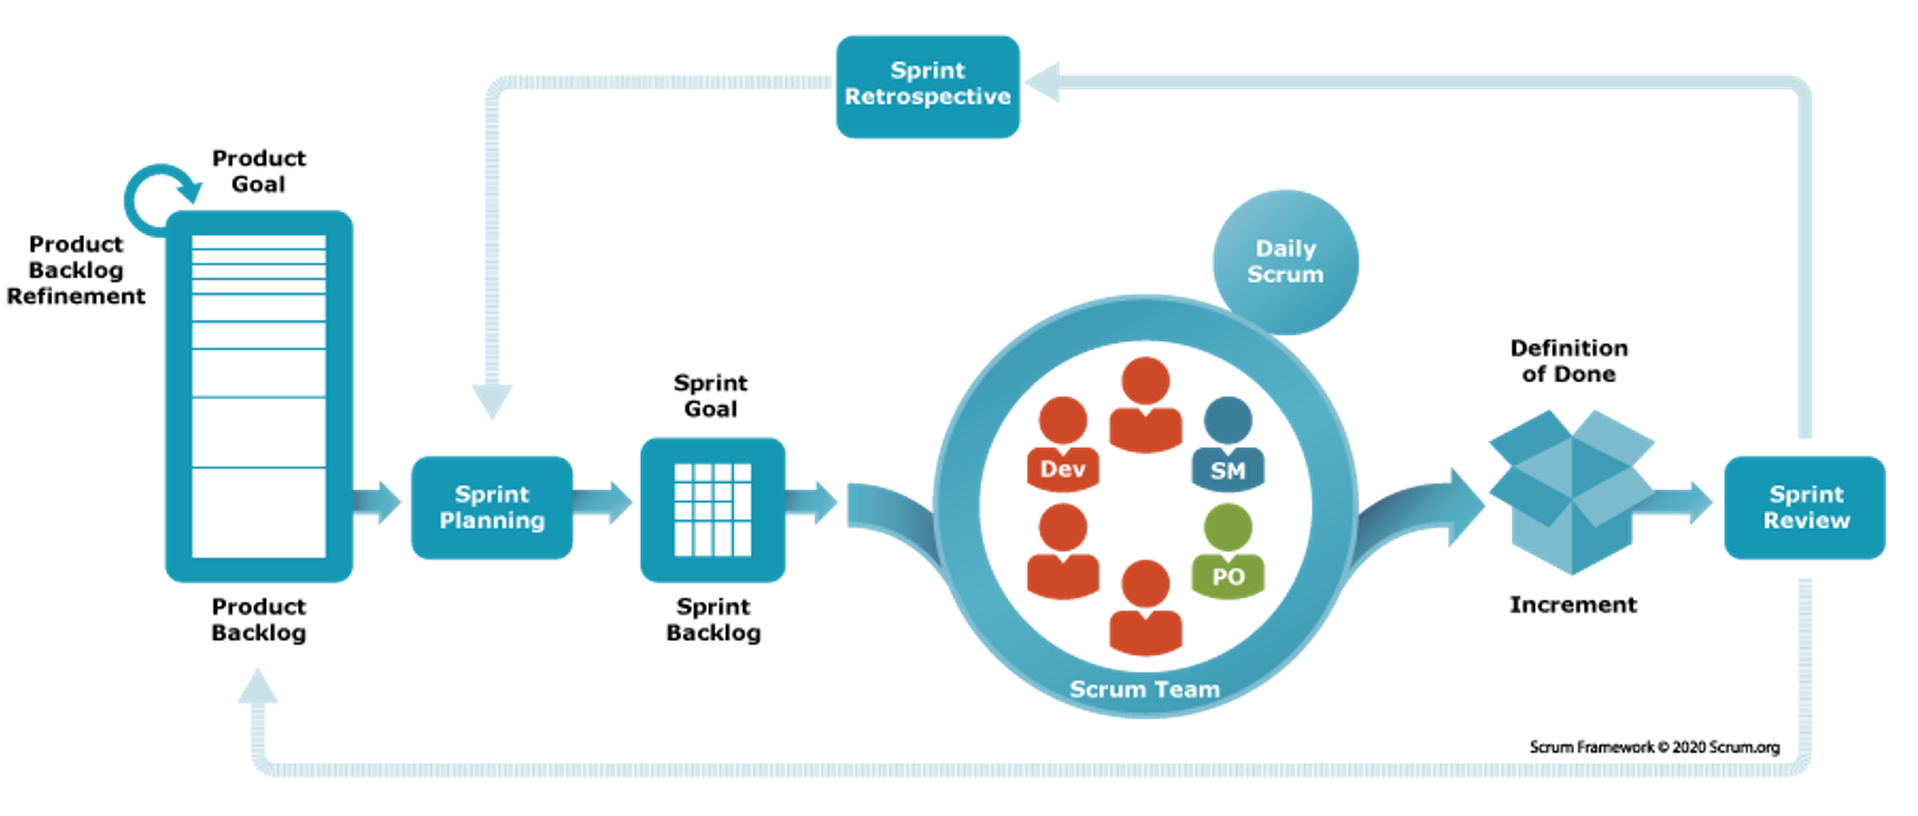
\includegraphics[width=0.9\textwidth]{./img/methodologies/scrum.png}
\caption{Esquema de funcionamiento de Scrum.}
\label{fig:scrum}
\vspace{0.2em}
{\footnotesize \centering \textit{Fuente:} \url{https://www.scrum.org/learning-series/what-is-scrum/} \par}
\end{figure}

\paragraph{Kanban.} Esta metodología utiliza un tablero visual (\textit{Tablero Kanban}) para representar el flujo de trabajo. Las tareas se representan como tarjetas que se mueven por columnas como \textit{Por hacer}, \textit{En progreso} y \textit{Terminado}. Se establece un límite de trabajo en curso (WIP: Work In Progress, trabajo en progreso) para evitar sobrecargas. Kanban permite detectar cuellos de botella, optimizar procesos y mejorar de forma continua la eficiencia del equipo.

\paragraph{Extreme Programming (XP).} XP enfatiza la mejora continua y la satisfacción del cliente. Reduce riesgos mediante prácticas técnicas rigurosas:

\begin{enumerate}
    \item Desarrollo iterativo con entregas frecuentes de software funcional.
    \item Pruebas constantes (TDD: Test-Driven Development, desarrollo guiado por tests).
    \item Programación en pareja. Dos desarrolladores trabajan simultáneamente en la misma tarea con el propósito de reducir errores y mejorar el aprendizaje del equipo.
    \item Integración continua.
    \item Código simple y funcional.
    \item Retroalimentación rápida del cliente. El cliente está presente de manera frecuente en el proceso de desarrollo y proporciona su punto de vista para ajustar el desarrollo a sus necesidades
\end{enumerate}

\section{Diseño de la interfaz}

La interfaz ha sido diseñada siguiendo principios de \textbf{UX/UI centrados en la simplicidad, accesibilidad y claridad visual}. Se han creado prototipos en \textbf{Figma}, permitiendo iterar sobre la estructura de navegación, la jerarquía visual y la organización de las secciones: listas, recetas e invitados.

\section{Herramientas de testeo}

Durante el desarrollo se ha planificado el uso de diferentes tipos de pruebas con herramientas específicas según el nivel:

\begin{table}[H]
\centering
\begin{tabular}{|l|l|p{8cm}|}
\hline
\textbf{Tipo de Test} & \textbf{Herramientas} & \textbf{Descripción} \\
\hline
Unitarios & JUnit4, MockK & Pruebas de lógica de negocio y mocking de dependencias. \\
UI (Compose) & \texttt{ui-test-junit4} & Verificación de componentes de interfaz. \\
Integración & Firebase Emulator Suite, Fake Repositories + Hilt & Pruebas aisladas de servicios y flujo de datos. \\
End-to-End (E2E) & Espresso, Firebase Emulator Suite & Automatización de flujos de usuario completos. \\
Cobertura & Jacoco & Generación de informes de cobertura. \\
\hline
\end{tabular}
\caption{Resumen de herramientas de testeo utilizadas}
\label{tab:testing-tools}
\end{table}

Estas herramientas permiten asegurar que la aplicación cumple sus requisitos funcionales y no funcionales, y que es robusta frente a cambios \cite{android-testing, firebase-emulator, jacoco}.